\subsection{Signal Model}

\begin{frame}[t]{Signal model}

    % Sound propagation process $\Leftrightarrow$ Source $\to$ Filter $\to$ Receiver model

    For one source and $I$ microphones:

    \begin{equation*}
        \tikzmarknode{x}{\contMic}_i(t)
                = (
                    \textcolor{orange}{\tikzmarknode{h}{\contRIR}_i}
                    \tikzmarknode{A}{\contConv}
                    \tikzmarknode{s}{\contSrc})(t)
                    + \tikzmarknode{n}{\contNse}(t)
                    \quad i \in I
    \end{equation*}

    % $\contMic_i$, $i$-th microphone signal $\contSrc$ source, signal $\contRIR_i$, $i$-th Room Impulse Response $\contConv$, continuous convolution

    % \vspace{5mm}
    % \begin{columns}[T,onlytextwidth]
    %     \begin{column}{0.48\textwidth}
    %         \centering
    %         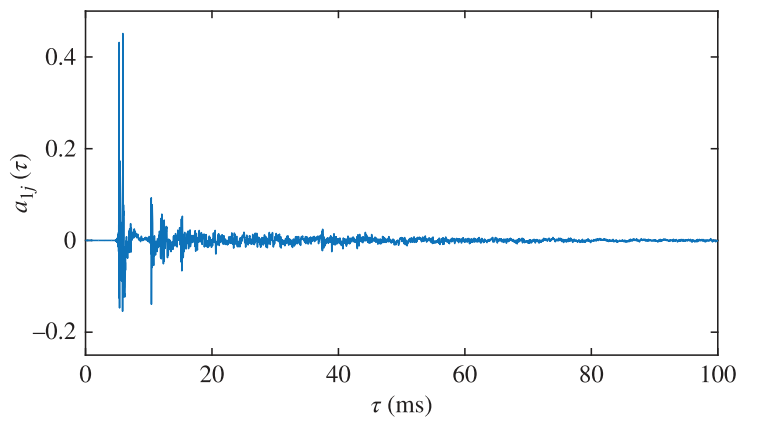
\includegraphics[width=\textwidth]{figures/rir_measured.png}
    %     \end{column}
    %     \begin{column}{0.48\textwidth}
    %         \centering
    %         \includegraphics<2>[width=\textwidth]{figures/rir_bang.png}
    %         \includegraphics<3->[width=\textwidth]{figures/rir_schematic.png}
    %     \end{column}
    % \end{columns}

    \begin{mydefblock}{\tikzmarknode{RIR}{Room Impulse Response} (RIR)}
        \small
        \begin{itemize}
            \item linear filtering effect of the sound
            \item acoustic response of a room to a (prefect) impulsive sound
            \item depends on spatial properties (room geometry, mic/src position)
            \item $\contRIR_i \neq \contRIR_j$
        \end{itemize}
    \end{mydefblock}


    \begin{tikzpicture}[overlay,remember picture,
        nodes={inner sep=1pt, align=center, font=\footnotesize},
        gray!70,>=stealth] %
    \draw[->] (x.north) to[out=90, in=0]   ++ (-8mm,+4mm) node[left] {{mic. signal}};
    \draw[->] (s.north) to[out=90, in=180] ++ (+8mm,+4mm) node[right] {{source signal}};
    \draw[->] (n.south) to[out=-90, in=180] ++ (+8mm,-4mm) node[right] {{noise term}};
    \draw[->] (A.south) to[out=-90, in=180] ++ (+8mm,-8mm) node[right] {{\faExclamationTriangle~continuous-time convolution}};
    \draw[->] (h.south) to[out=-90, in=90] (RIR.north);
    \end{tikzpicture}


    \begin{columns}
        \column{0.48\textwidth}
            \centering
            % real RIR with part
            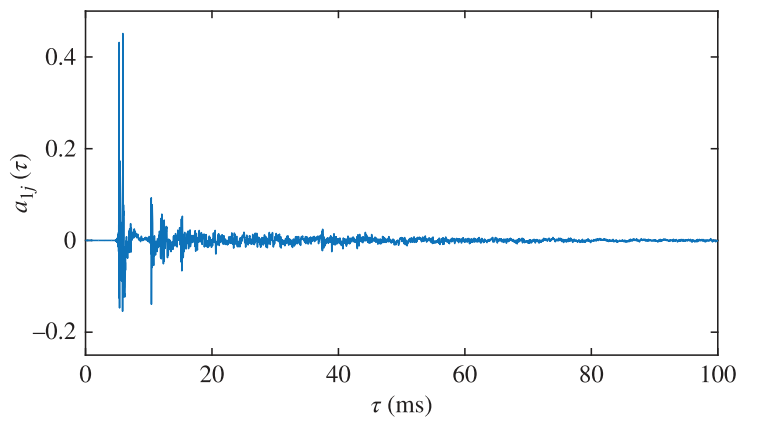
\includegraphics[width=0.8\textwidth]{figures/rir_measured.png}

        \column{0.48\textwidth}
            \centering
            % bang RIR
            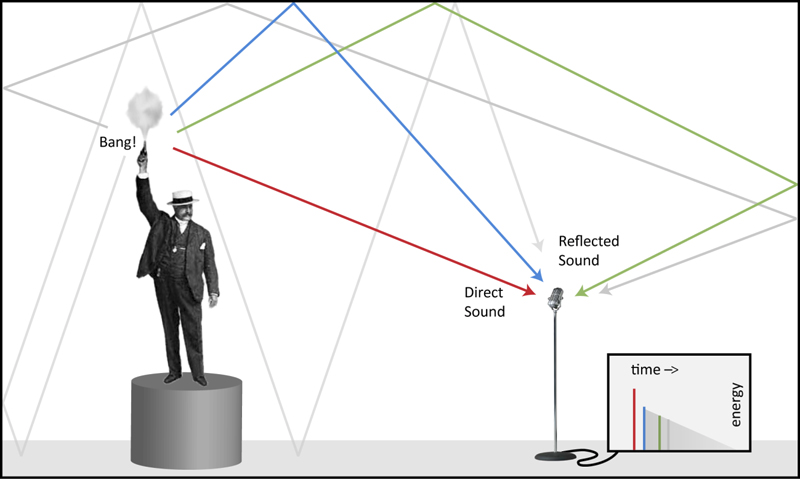
\includegraphics[width=0.8\textwidth]{figures/rir_bang.png}

    \end{columns}

\end{frame}


\subsection{Current Challenges}

\begin{frame}{Problem Statement}
    \begin{columns}[T,onlytextwidth]
        \column{0.48\textwidth}
        \begin{equation*}
            \begin{aligned}
                \contMic_i(t) &= (\contRIR_i \contConv \contSrc)(t) + \contNse(t)\\
                \contRIR_i(t) &= \textcolor{myred}{\contRIRidirect}(t)
                              + \textcolor{myblue}{\contRIRiearly}(t)
                              + \textcolor{mygreen}{\contRIRilate}(t)

            \end{aligned}
        \end{equation*}
        \begin{itemize}\small
            \item $\textcolor{myred}{\contRIRidirect}(t)$ = direct path
            \item $\textcolor{myblue}{\contRIRiearly}(t)$ = early reflection
            \item $\textcolor{mygreen}{\contRIRilate}(t)$ = late reverberation
        \end{itemize}

        \column{0.48\textwidth}
        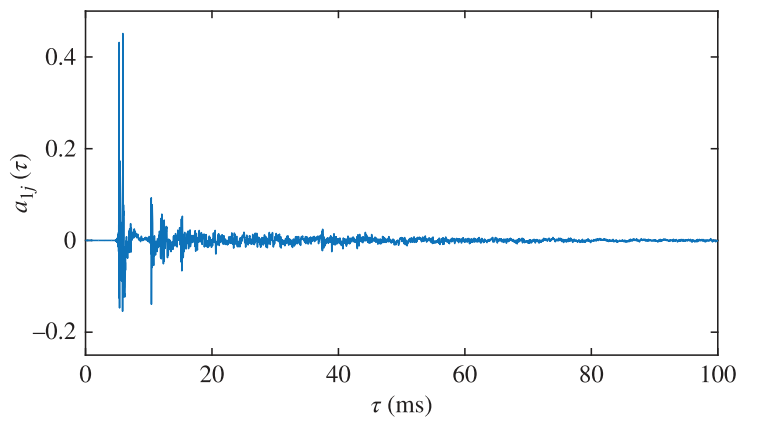
\includegraphics[width=.8\textwidth]{figures/rir_measured.png}

    \end{columns}

    Echoes can be modeled as sum of Dirac's delta function:

    \begin{equation*}
        \contRIR_i(t) =
            \textcolor{myred}{\contRIRidirect}(t) + \textcolor{myblue}{\contRIRiearly}(t) + \varepsilon_i(t)
            \approx \sum_{r=0}^{R} \ampir \delta(t - \textcolor{alert}{\tauir}) + \tikzmarknode{error}{\varepsilon}_i(t)
    \end{equation*}

    \begin{textblock*}{20mm}(100mm,60mm)
        \footnotesize
        \tikzmarknode{model}{models} later echoes, reverberation and other.
    \end{textblock*}


    \begin{tikzpicture}[overlay,remember picture,
        nodes={inner sep=1pt, align=center, font=\footnotesize},
        gray!70,>=stealth] %
    \draw[->] (error.north) to[out=-90, in=180] (model.west);
    \end{tikzpicture}


    \begin{mydefblock}{Goals: Acoustic Echo Retrieval (AER)}
        Estimated $\set{\alert{\tauir}, \ampir_i}_{i,r}$
        for the microphone signal $\set{x_i}_i$
    \end{mydefblock}
    \addendum{\scriptsize {Estimation of only $\tauir$ is known as TOAs estimation}}

\end{frame}


\begin{frame}{Problem Statement}

    \begin{mydefblock}{Goals: Acoustic Echo Retrieval (AER)}
        Estimated $\set{\alert{\tauir}, \ampir_i}_{i,r}$
        for the microphone signal $\set{x_i}_i$
    \end{mydefblock}

    \textbf{Challenges:}
    \begin{itemize}
        \item RIRs depend on the scene geometry (room, source and mic position)
        \item Big under-modelling error
        \begin{itemize}
            \item in the RIR model due to late reverberation
            \item in the signal model due to interferences and noise
        \end{itemize}
        \item $\ampir$ are distorted:
        \begin{itemize}
            \item $\ampir \to \ampir(t)$ (e.g. air attenuation, wall absorption)
            \\\hspace{.5em}$\implies$ echo model is sum of filters
            \item sampling process{\footnotesize~\cite{tukuljac2018mulan}}
        \end{itemize}
    \end{itemize}

    \begin{center}
        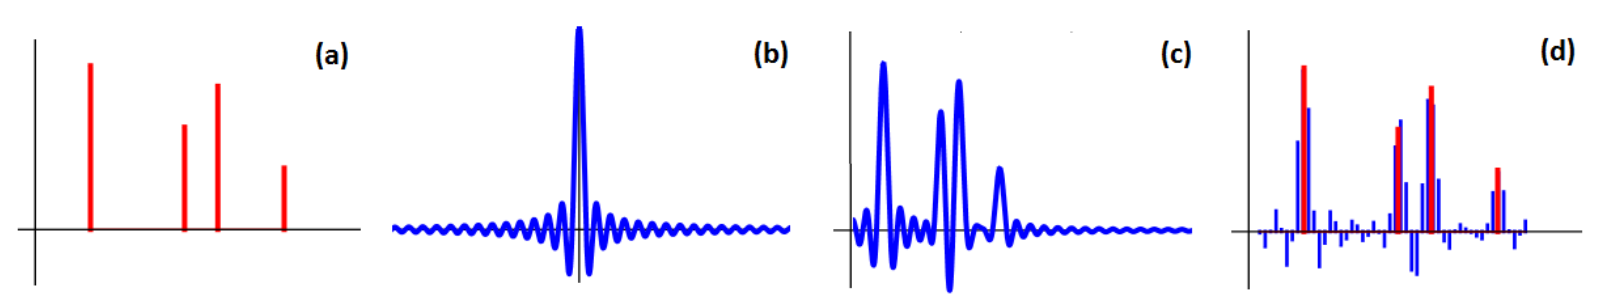
\includegraphics[width=0.8\textwidth]{figures/basismismatch.png}
        \\{\addendum{\scriptsize Courtesy of Helena Tukuljac~\cite{tukuljac2018mulan}}}
    \end{center}

\end{frame}